\subsection{Celebrity Faces} \label{sec:celeba}

%\newcommand{\thirdFigWidth}{0.15\textwidth}

\begin{figure}[ht!]
%
% \begin{center}
% \centering
\begin{subfigure}[t]{\thirdFigWidth}
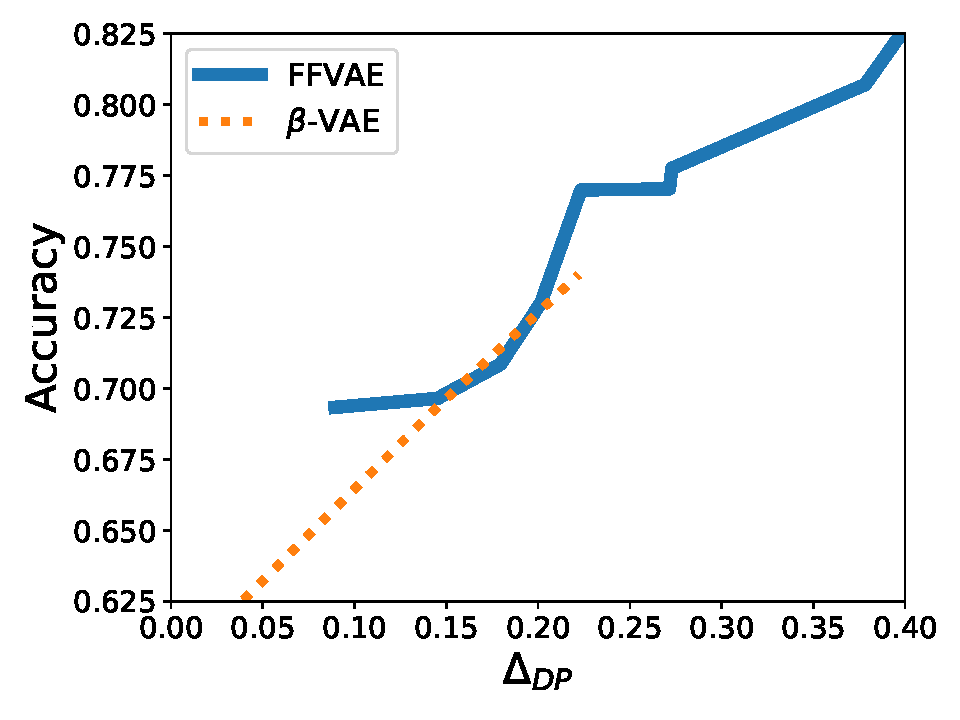
\includegraphics[width=\textwidth]{predict_C.pdf}
\caption{$a$ = C}
\label{fig:predict_C}
\end{subfigure}
%
\hfill
%
\begin{subfigure}[t]{\thirdFigWidth}
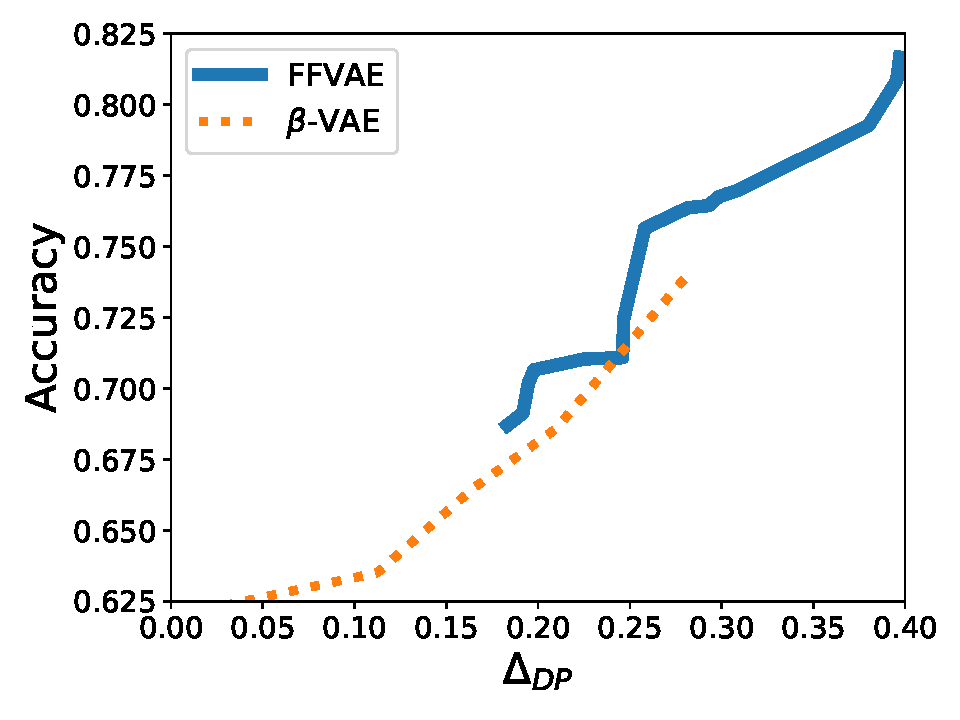
\includegraphics[width=\textwidth]{predict_E.pdf}
\caption{$a$ = E}
\label{fig:predict_E}
\end{subfigure}
%
\hfill
%
\begin{subfigure}[t]{\thirdFigWidth}
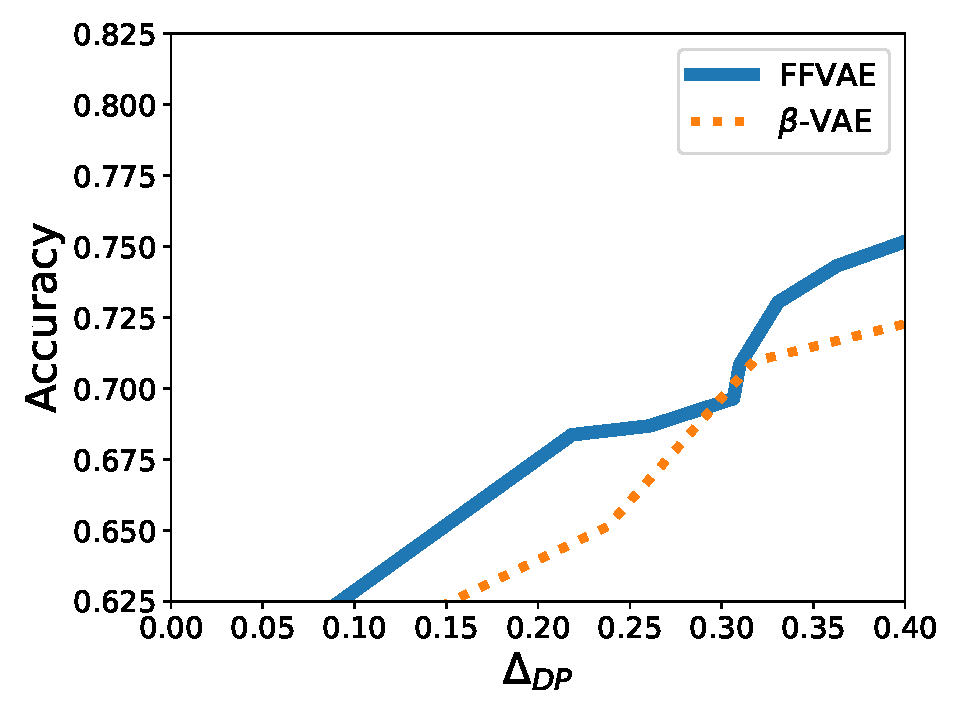
\includegraphics[width=\textwidth]{predict_M.pdf}
\caption{$a$ = M}
\label{fig:predict_M}
\end{subfigure}
%
\hfill
%
\begin{subfigure}[t]{\thirdFigWidth}
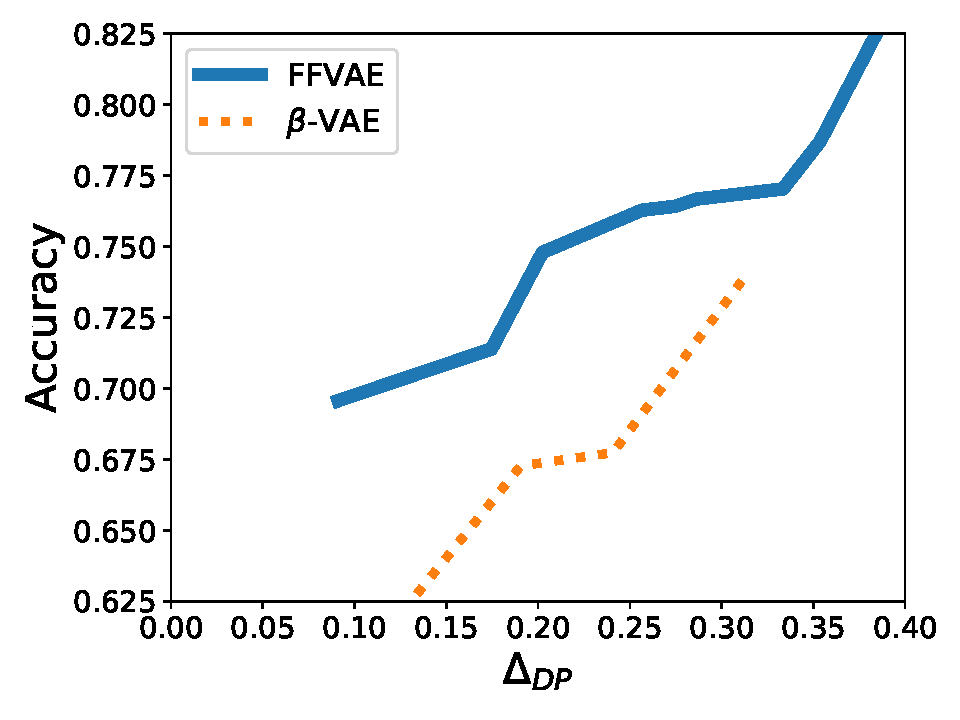
\includegraphics[width=\textwidth]{predict_C-AND-E.pdf}
\caption{$a$ = C $\wedge$ E}
\label{fig:predict_C-AND-E}
\end{subfigure}
%
\hfill
%
\begin{subfigure}[t]{\thirdFigWidth}
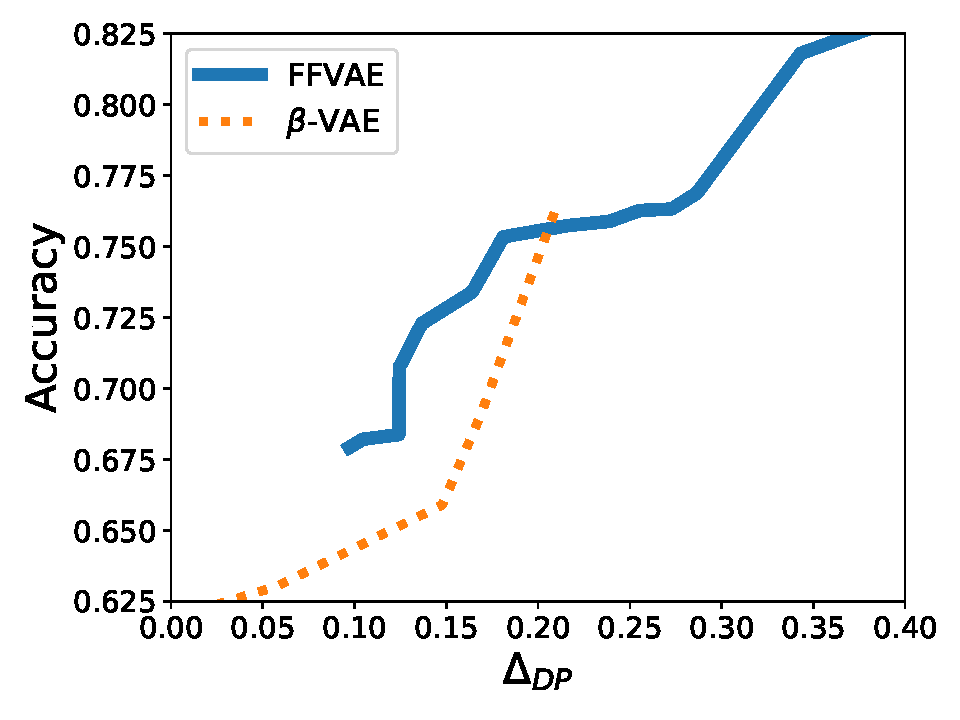
\includegraphics[width=\textwidth]{predict_C-AND-NOT-E.pdf}
\caption{$a$ = C $\wedge \neg$ E}
\label{fig:predict_C-AND-NOT-E}
\end{subfigure}
%
\hfill
%
\begin{subfigure}[t]{\thirdFigWidth}
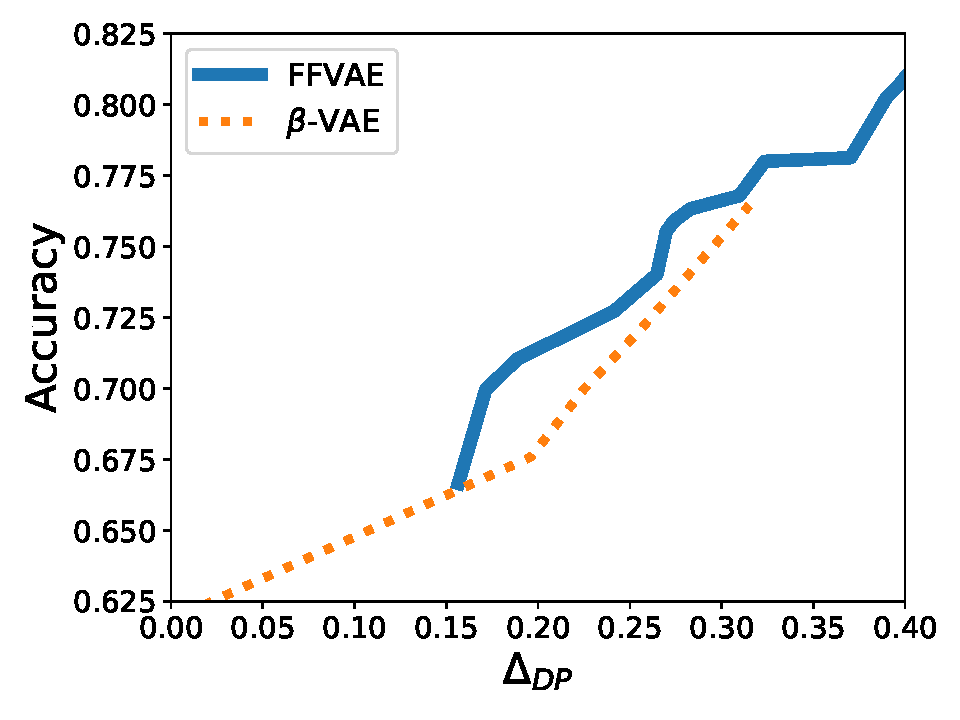
\includegraphics[width=\textwidth]{predict_NOT-C-AND-E.pdf}
\caption{$a$ = $\neg$ C $\wedge$ E}
\label{fig:predict_NOT-C-AND-E}
\end{subfigure}
%
\hfill
%
\begin{subfigure}[t]{\thirdFigWidth}
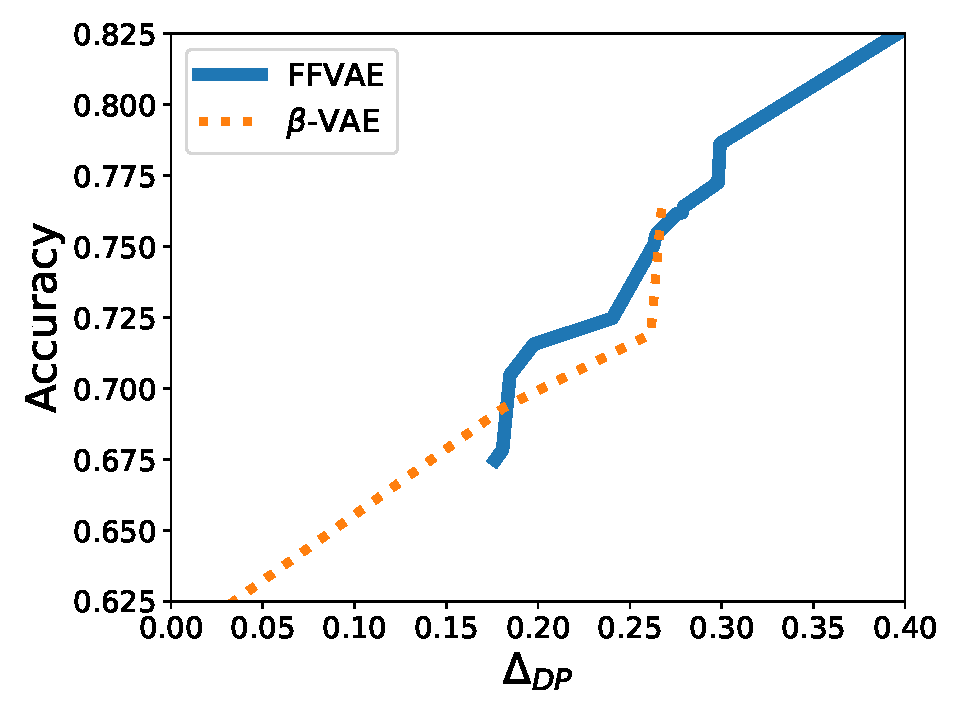
\includegraphics[width=\textwidth]{predict_NOT-C-AND-NOT-E.pdf}
\caption{$a$ = $\neg$ C $\wedge \neg$ E}
\label{fig:predict_NOT-C-AND-NOT-E}
\end{subfigure}
%
\hfill
%
\begin{subfigure}[t]{\thirdFigWidth}
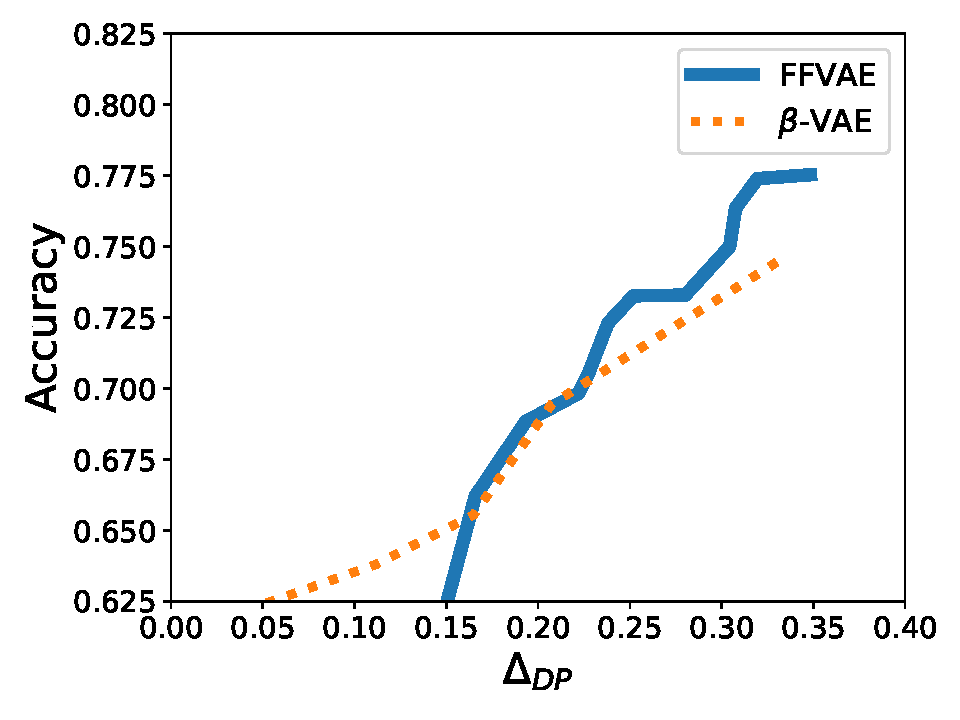
\includegraphics[width=\textwidth]{predict_C-AND-M.pdf}
\caption{$a$ = C $\wedge$ M}
\label{fig:predict_C-AND-M}
\end{subfigure}
%
\hfill
%
\begin{subfigure}[t]{\thirdFigWidth}
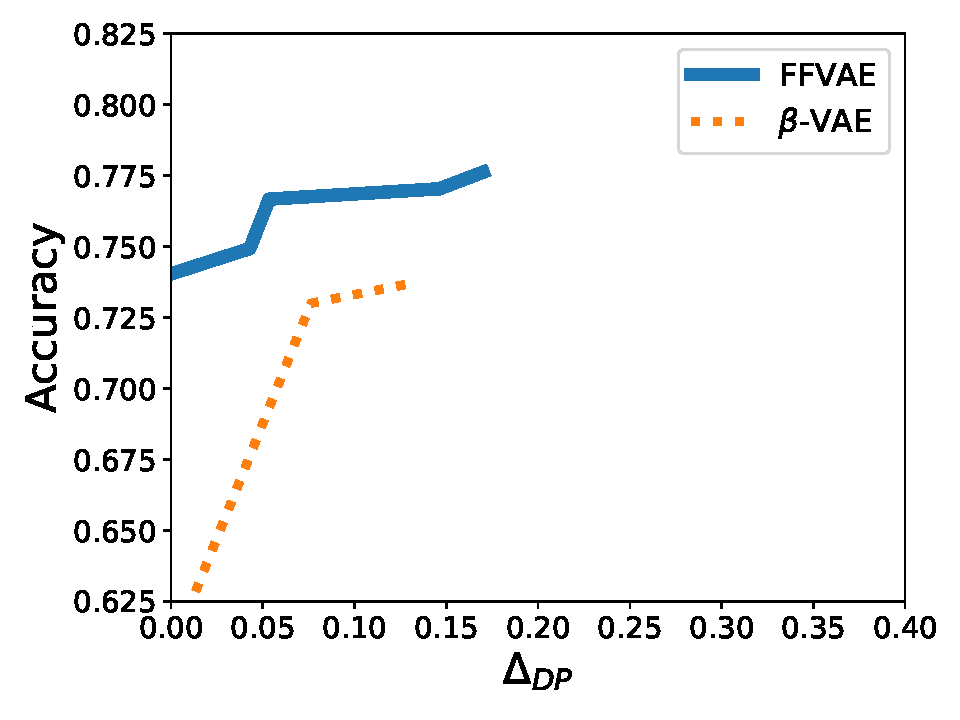
\includegraphics[width=\textwidth]{predict_C-AND-NOT-M.pdf}
\caption{$a$ = C $\wedge \neg$ M}
\label{fig:predict_C-AND-NOT-M}
\end{subfigure}
%
\hfill
%
\begin{subfigure}[t]{\thirdFigWidth}
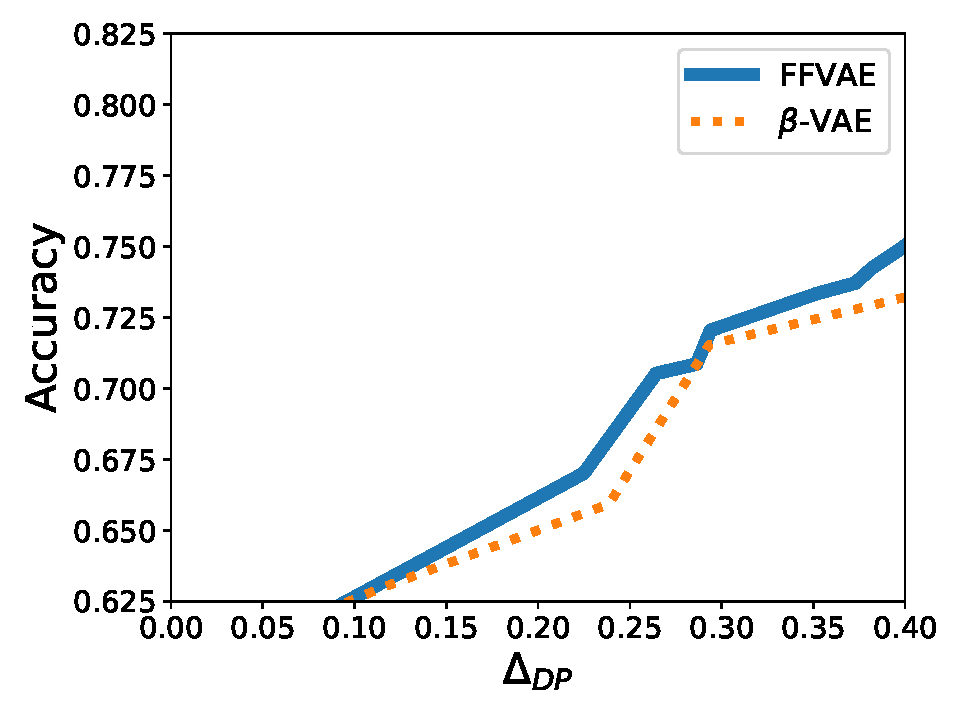
\includegraphics[width=\textwidth]{predict_NOT-C-AND-M.pdf}
\caption{$a$ = $\neg$ C $\wedge$ M}
\label{fig:predict_NOT-C-AND-M}
\end{subfigure}
%
\hfill
%
\begin{subfigure}[t]{\thirdFigWidth}
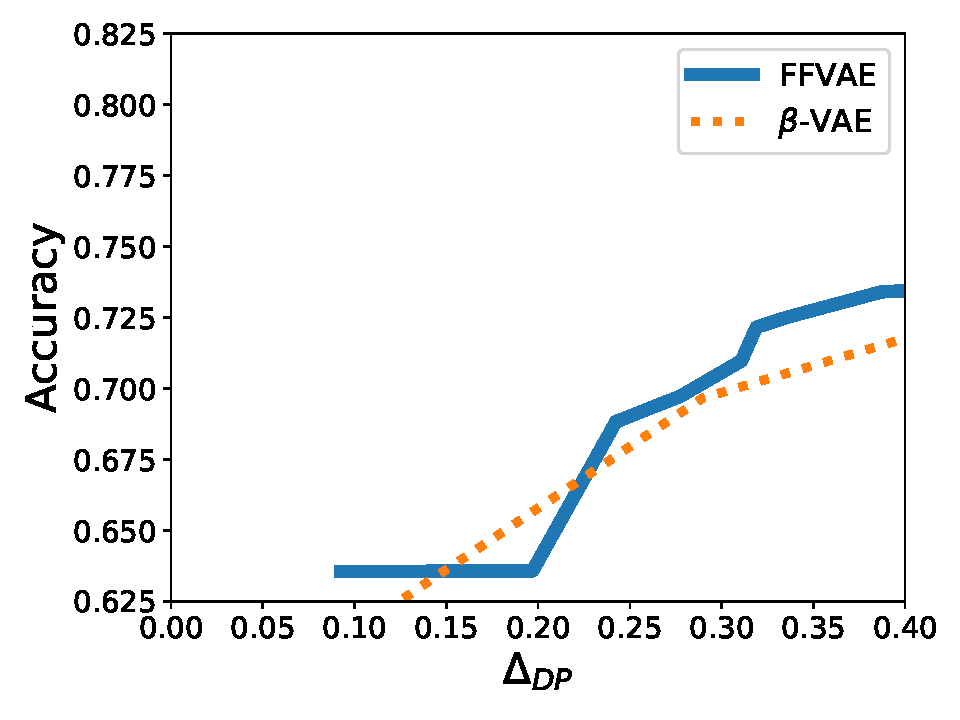
\includegraphics[width=\textwidth]{predict_NOT-C-AND-NOT-M.pdf}
\caption{$a$ = $\neg$ C $\wedge \neg$ M}
\label{fig:predict_NOT-C-AND-NOT-M}
\end{subfigure}
%
\hfill
%
\begin{subfigure}[t]{\thirdFigWidth}
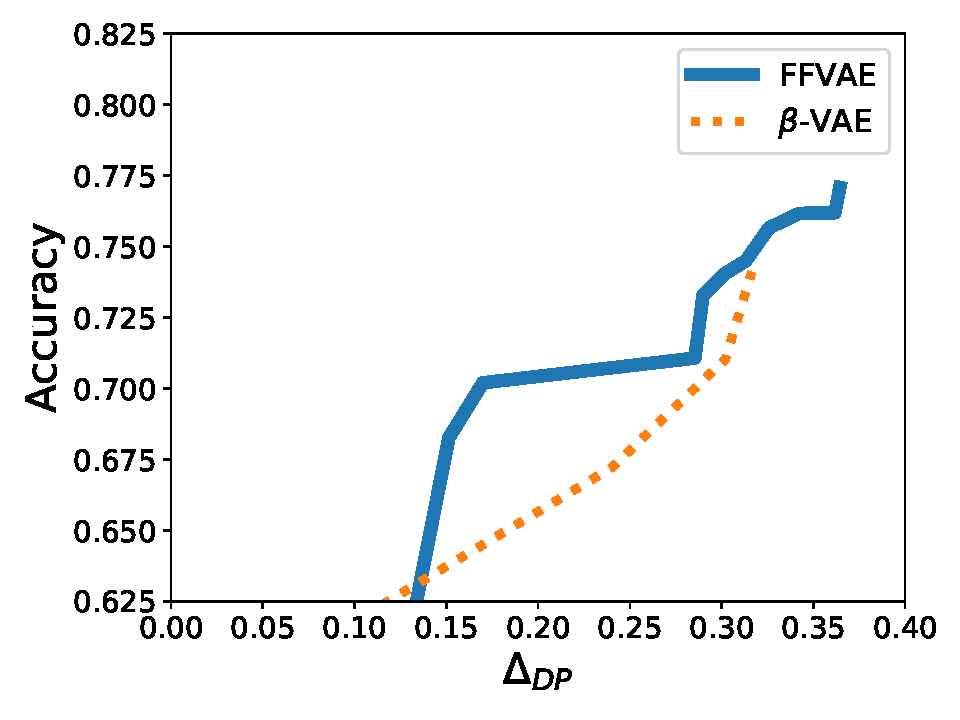
\includegraphics[width=\textwidth]{predict_E-AND-M.pdf}
\caption{$a$ = $\neg$ E $\wedge$ M}
\label{fig:predict_E-AND-M}
\end{subfigure}
%
\hfill

%
\begin{subfigure}[t]{\thirdFigWidth}
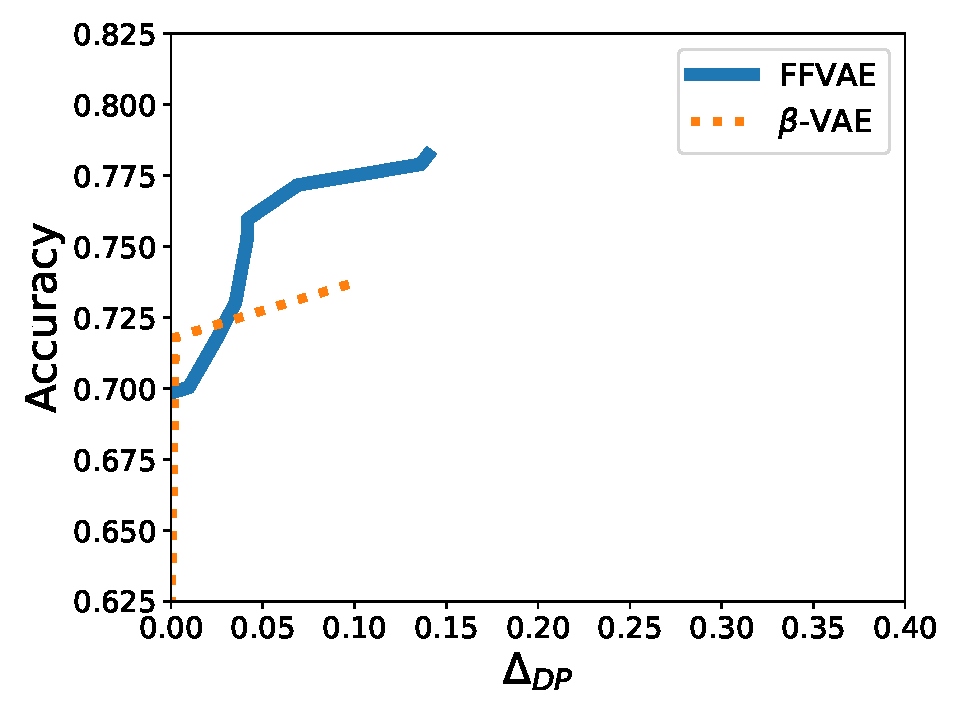
\includegraphics[width=\textwidth]{predict_E-AND-NOT-M.pdf}
\caption{$a$ = E $\wedge \neg$ M}
\label{fig:predict_E-AND-NOT-M}
\end{subfigure}
%
\hfill
%
\begin{subfigure}[t]{\thirdFigWidth}
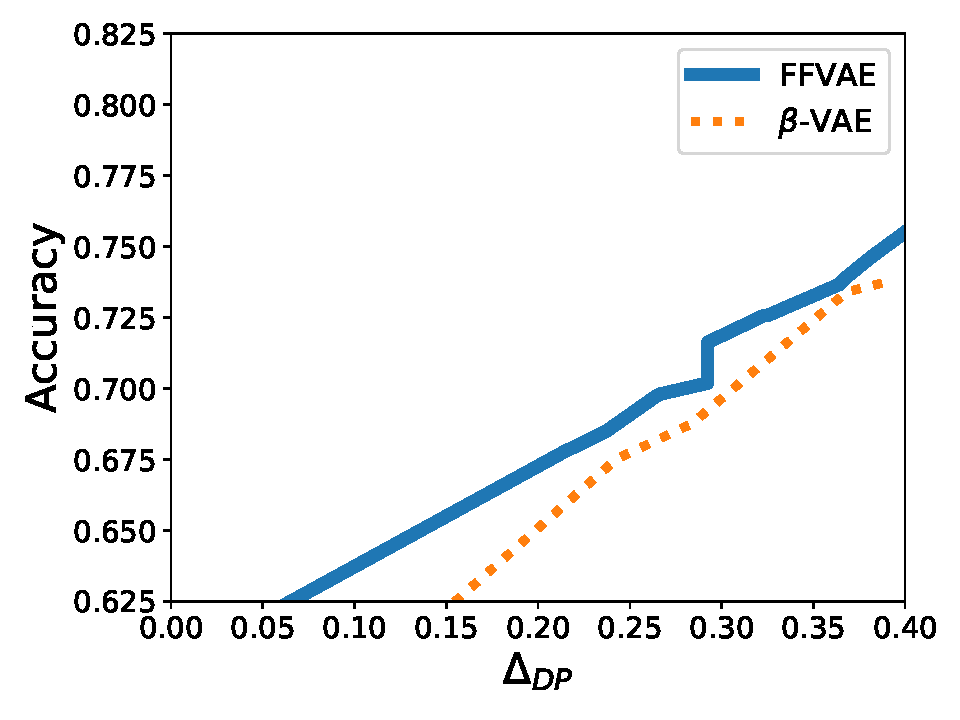
\includegraphics[width=\textwidth]{predict_NOT-E-AND-M.pdf}
\caption{$a$ = $\neg$ E $\wedge$ M}
\label{fig:predict_NOT-E-AND-M}
\end{subfigure}
%
\hfill
%
\begin{subfigure}[t]{\thirdFigWidth}
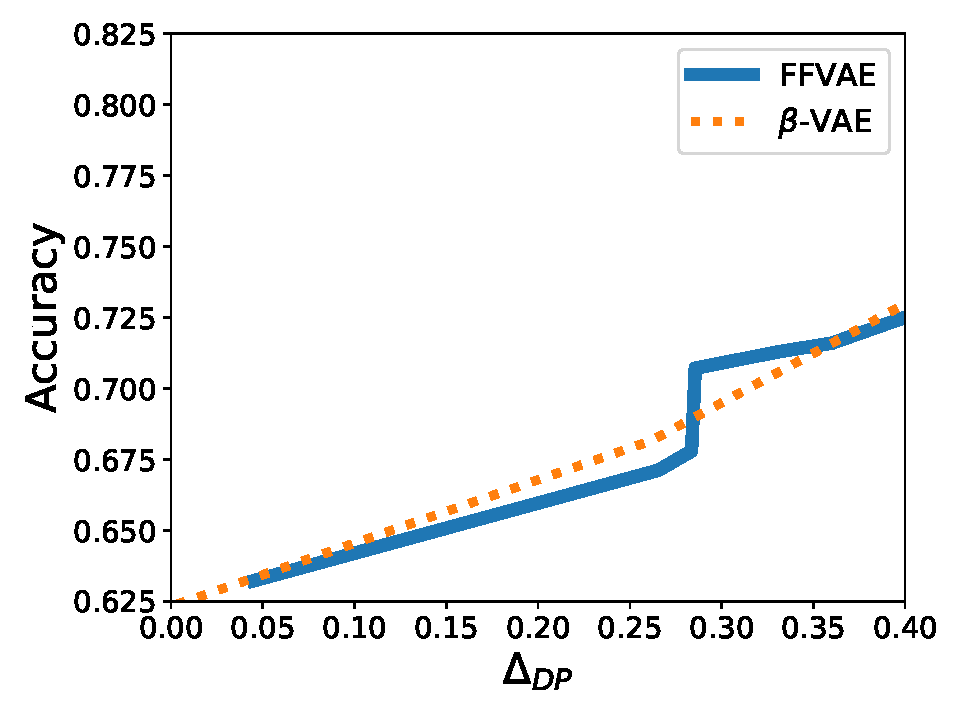
\includegraphics[width=\textwidth]{predict_NOT-E-AND-NOT-M.pdf}
\caption{$a$ = $\neg$ E $\wedge \neg$ M}
\label{fig:predict_NOT-E-AND-NOT-M}
\end{subfigure}
%
\hfill

\caption{
    Celeb-A subgroup fair classification results.
    Sensitive attributes: Chubby (C), Eyeglasses (E), and Male (M).
    $y$ = HeavyMakeup. 
    }
    \label{fig:celeba-pareto}
% \end{center}
% \vskip -0.2in
\end{figure}


\paragraph{Dataset}
The CelebA\footnote{\scriptsize \url{http://mmlab.ie.cuhk.edu.hk/projects/CelebA.html}} dataset contains over $200,000$ images of celebrity faces.
Each image is associated with 40 human-labeled binary attributes (OvalFace, HeavyMakeup, etc.).
We chose three attributes, Chubby, Eyeglasses, and Male as sensitive attributes\footnote{
We chose these attributes because they co-vary relatively weakly with each other (compared with other attribute triplets), but strongly with other attributes.
Nevertheless the rich correlation structure amongst all attributes makes this a challenging fairness dataset; it is difficult to achieve high accuracy and low $\Delta_{DP}$.
}, and report fair classification results on 3 groups and 12 two-attribute-conjunction subgroups only (for brevity we omit three-attribute conjunctions).
To our knowledge this is the first exploration of fair representation learning algorithms on the Celeb-A dataset.
As in the previous sections we train the encoders on the train set, then evaluate performance of MLP classifiers trained on the encoded test set.

\paragraph{Fair Classification}

We follow the fair classification audit procedure described above, where the held-out label HeavyMakeup---which was not used at encoder train time---is predicted by an MLP from the encoder representations.
When training the MLPs we take a fresh encoder sample for each minibatch (statically encoding the dataset with one encoder sample per image induced overfitting).
We found that training the MLPs on encoder means (rather than samples) increased accuracy but at the cost of very unfavorable $\Delta_{DP}$.
We also found that FactorVAE-style adversarial training does not scale well to this high-dimensional problem, so we instead optimize Equation \ref{eq:ffvae} using the biased estimator from \citet{chen2018isolating}.
Figure \ref{fig:celeba-pareto} shows Pareto fronts that capture the fairness-accuracy tradeoff for FFVAE and $\beta$-VAE.

While neither method dominates in this challenging setting, FFVAE achieves a favorable fairness-accuracy tradeoff across many of subgroups.
We believe that using sensitive attributes as side information gives FFVAE an advantage over $\beta$-VAE in predicting the held-out label.
In some cases (e.g., $a$=$\neg$E$\wedge$M) FFVAE achieves better accuracy at all $\Delta_{DP}$ levels, while in others (e.g., $a$=$\neg$C$\wedge\neg$E)
, FFVAE did not find a low-$\Delta_{DP}$ solution.
We believe Celeb-A--with its many high dimensional data and rich label correlations---is a useful test bed for subgroup fair machine learning algorithms, and we are encouraged by the reasonably robust performance of FFVAE in our experiments.
